\documentclass[12pt]{article}

\usepackage{amsmath}
\usepackage{graphicx}
\usepackage{svg}
\usepackage{float}
\usepackage{longtable} 
\usepackage{circuitikz}
\usepackage[margin=1.2in]{geometry}


\begin{document}
\title{Sub-Group: A-7 \\ Experiment 2: Study of Transistor Characteristics}


\author{Sayan Karmakar \\22MS163 }
\date{}
\maketitle

\section{Aim}
To study input and output charecterestics of a common-emmiter configuration of a npn BJT transistor.

\section{Theory}
Transistors are a very common and useful device in modern days. It is used as oscillators, amplifiers, gates and many other instruments. One of the common type transistors are bipolar junction transistor. This bipolar junction transistor is a sandwich of semiconducting materials. In an npn transistor there is a p-type semiconductor in between two n-type semiconductors. And in a pnp transistor there is a n-type semiconductor in between two p-type semiconductors. In this experiment, we are going to study the input and output characteristics of npn semiconductors.

In an npn semiconductor, out of the two n-type semiconductors one of them is very heavily doped and the other is larger in size and lightly doped compared to the other n-type. The heavily doped semiconductor is called Emitter. The comparatively lightly doped semiconductor is called Collector. The p-type semiconductor is generally very thin and very lightly doped. There are two pn junctions present in the transistor - base emitter junction and the collector base junction. Normally when used as an amplifier, the base emitter junction is kept in forward bias and the collector base junction is kept in reverse bias. So, due to the forward bias of the base emitter junction electrons go from emitter to the base, this electrons get affected by the reverse bias of the collector base junction and as the base is very thin and lightly doped most of the electrons go to the collector. So the emitter current is almost equal to the collector current. It is actually slightly more than the emitter current. We define a parameter \( \alpha \) as 

\begin{equation*}
\mathrm{I_C = \alpha I_E}
.\end{equation*}
\( \alpha \) is slightly smaller than 1. We can write also \( \mathrm{I_E = I_C + I_B}\). So if we define \( \beta \) as \( \mathrm{I_C = \beta I_B} \) then we can write 

\begin{equation*}
\beta = \frac{\alpha}{(1 - \alpha)} 
\end{equation*}

Now as the transistor is a three terminal device one of the terminals has to be considered as a common terminal while studying input or output characteristics. Depending on the terminal we can define three types of configuration - common emitter configuration, common base, common collector configuration. This experiment concerns only common emitter configuration.
\begin{figure}[!ht]
    \centering
    \resizebox{0.7\textwidth}{!}{%
    \begin{circuitikz}
    \tikzstyle{every node}=[font=\normalsize]
    \draw (4,14) to[short] (6,14);
    \draw (4,14) to[short] (4,12.5);
    \draw (4,12.5) to[battery ,l={ \normalsize $\mathrm{V_{BB}}$}] (4,11.25);
    \draw (4,11.25) to[short] (4,10);
    \draw (4,10) to[short] (9.75,10);
    \draw  (6.5,14) circle (0.5cm) node {\normalsize $\mu \mathrm{A}$} ;
    \draw (7,14) to[R,l={ \normalsize $\mathrm{R_B}$}] (9,14);
    \draw (10,13) to[Tnpn, transistors/scale=1.19] (10,15);
    \draw  (10,14) circle (1cm);
    \draw [short] (10,13) -- (10,10);
    \draw [short] (9.75,10) -- (16.5,10);
    \draw [short] (10,15) -- (10,16);
    \draw [short] (10,16) -- (12,16);
    \draw (12,16) to[R,l={ \normalsize $\mathrm{R_C}$}] (14.25,16);
    \draw  (15.25,16) circle (0.5cm) node {\normalsize mA} ;
    \draw (14.25,16) to[short] (14.75,16);
    \draw (15.75,16) to[short] (16.5,16);
    \draw (16.5,16) to[battery ,l={ \normalsize $\mathrm{V_{CC}}$}] (16.5,10);
    \draw (11.75,16) to[short] (11.75,13);
    \draw  (11.75,12.5) circle (0.5cm) node {\normalsize $\mathrm{V_{CE}}$} ;
    \draw (11.75,12) to[short] (11.75,10);
    \node [font=\normalsize] at (6.5,14.25) {};
    \draw (8.75,14) to[short] (8.75,13);
    \draw  (8.75,12.5) circle (0.5cm) node {\normalsize $\mathrm{V_{BE}}$} ;
    \draw (8.75,12) to[short] (8.75,10);
    \end{circuitikz}
    }%
    \caption{Circuit Diagram}
    \label{fig:my_label}
    \end{figure}

\begin{figure}[H]
    \centering
    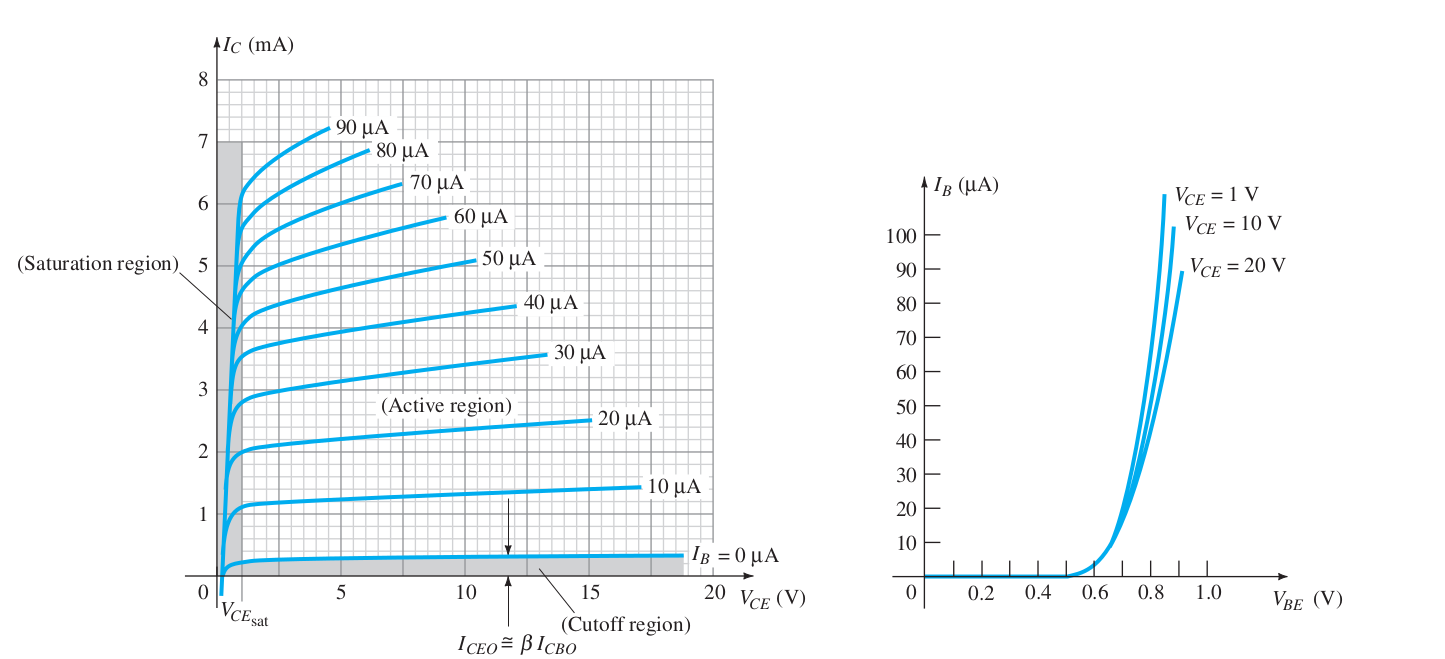
\includegraphics[width = \textwidth]{IN_OUT.png}
    \caption{Output and Input Characterestics of an ideal Transistor}
    \label{fig:char}
\end{figure}
For studying three terminal devices two sets of characteristics are necessary. Input characteristics is the study of dependency of input current (\( \mathrm{I_B} \)) and base emitter voltage (\( \mathrm{V_{BE}} \)) while keeping the collector current (\( \mathrm{I_C}\)) fixed and the output characteristics is the study of collector current(\( \mathrm{I_C }\)) and base collector voltage (\( \mathrm{V_{CE}} \)) fixed while keeping the base current (\( \mathrm{I_B } \)) fixed.



\section{Data and Calculation}

\subsection{Input Characteristics}

Firstly we made the circuit with \(\mathrm{R_B = 1 k\Omega}\) and \( \mathrm{R_C = 1 \Omega }\). In the following two tables we noted down the values of necessary quantities for studying input characteristics. For the first table we set the output voltage $\mathrm{V_{CE}}$ to be  2 V and in the next table we set the output voltage $\mathrm{V_{CE}}$ to be 3 V.  For these voltages, we took the measurements for the input voltage $\mathrm{V_{BE}}$ and the input current $\mathrm{I_B}$.

\begin{longtable}[H]{|c|c|c|c|c|c|}
    \caption{Table for \( \mathrm{V_{CE}} = 2\) V}
    \endfirsthead
    \hline
    $\mathrm{V_{BB} \ (V)}$ & $\mathrm{V_{BE} (V)}$ & $\mathrm{I_B (mA)}$ & $\mathrm{I_C (mA)}$ & $\mathrm{V_{CC} (V)}$ & $\mathrm{V_{CE} (V)}$ \\ \hline \hline
    \endhead
    \hline
    $\mathrm{V_{BB} \ (V)}$ & $\mathrm{V_{BE} (V)}$ & $\mathrm{I_B (mA)}$ & $\mathrm{I_C (mA)}$ & $\mathrm{V_{CC} (V)}$ & $\mathrm{V_{CE} (V)}$ \\ \hline \hline
    0         & 0.036     & 0            & 0            & 2     & 2             \\ \hline
    0.1       & 0.178     & 0            & 0            & 2     & 2             \\ \hline
    0.2       & 0.251     & 0            & 0            & 2     & 2             \\ \hline
    0.3       & 0.378     & 0            & 0            & 2     & 2             \\ \hline
    0.4       & 0.449     & 0            & 0            & 2     & 2             \\ \hline
    0.5       & 0.589     & 3            & 5            & 2     & 2             \\ \hline
    0.6       & 0.655     & 28           & 4.7          & 2     & 2             \\ \hline 
    0.7       & 0.698     & 91           & 16.3         & 2     & 2             \\ \hline
    0.8       & 0.729     & 182          & 32.6         & 2     & 2             \\ \hline
    0.9       & 0.738     & 226          & 41.1         & 2     & 2             \\ \hline
    1         & 0.762     & 338          & 61.6         & 2     & 2             \\ \hline 
    1.1       & 0.778     & 414          & 76.1         & 2     & 2             \\ \hline
    1.2       & 0.792     & 499          & 92.3         & 2     & 2             \\ \hline 
    
\end{longtable}


\begin{longtable}[H]{|c|c|c|c|c|c|}
    \caption{Table for \( \mathrm{V_{CE}} = 3\) V}
    \endfirsthead
    \hline
    $\mathrm{V_{BB} \ (V)}$ & $\mathrm{V_{BE} (V)}$ & $\mathrm{I_B (mA)}$ & $\mathrm{I_C (mA)}$ & $\mathrm{V_{CC} (V)}$ & $\mathrm{V_{CE} (V)}$ \\
    \hline \hline
    \endhead
    \hline
    $\mathrm{V_{BB} \ (V)}$ & $\mathrm{V_{BE} (V)}$ & $\mathrm{I_B (mA)}$ & $\mathrm{I_C (mA)}$ & $\mathrm{V_{CC} (V)}$ & $\mathrm{V_{CE} (V)}$ \\
    \hline \hline
    0     & 0.038 & 0            & 0            & 3     & 3             \\ \hline
    0.1   & 0.19  & 0            & 0            & 3     & 3             \\ \hline
    0.2   & 0.259 & 0            & 0            & 3     & 3             \\ \hline
    0.3   & 0.355 & 1            & 0            & 3     & 3             \\ \hline
    0.4   & 0.466 & 1            & 0            & 3     & 3             \\ \hline
    0.5   & 0.607 & 9            & 1.6          & 3     & 3             \\ \hline
    0.6   & 0.642 & 27           & 5            & 3     & 3             \\ \hline
    0.7   & 0.684 & 88           & 16.2         & 3     & 3             \\ \hline
    0.8   & 0.71  & 158          & 29.4         & 3     & 3             \\ \hline
    0.9   & 0.729 & 242          & 45.9         & 3     & 3             \\ \hline
    1     & 0.749 & 334          & 64.8         & 3     & 3             \\ \hline
    1.1   & 0.767 & 449          & 87.2         & 3     & 3             \\ \hline
    1.2   & 0.765 & 468          & 93           & 3     & 3             \\ \hline           
\end{longtable}

From the above graphs we plotted the following graph. The graph shows the input characteristics of the transistor that is the dependency of input voltage and input current for different output voltage. We expected that for output voltage 3 V the graph to lie on the right of the graph for output voltage 2 V. But from our graph we see that the graph corresponding to 3 V lies to the right of 2 V. This is opposite of what we expected.

\begin{figure}[H]
    \centering
    \includesvg[width = 0.9\textwidth]{./Graphs/Input.svg}
    \caption{Input Characteristics of the Transistor}
\end{figure}

\subsection{Output Characteristics}
The following tables contain data for studying the output characteristics. Here we tabulated the collector current $\mathrm{I_C}$ and output voltage $\mathrm{V_{CE}}$ for different values of input current $I_B$. We took data corresponding to three different values of $I_B$ 25 $\mu$A, 30 $\mu$A and 40 $\mu$A respectively. For the following data collection we set the resistance \( \mathrm{R_B = 220 \Omega }\) and the resistance \( \mathrm{R_C = 1 k \Omega}\).

\begin{longtable}[H]{|c|c|c|c|c|}
    \caption{Table for \( \mathrm{I_B}\) = 25 \( \mu \)A }
    \endfirsthead
    \hline   
    $\mathrm{V_{CC}}$ (V) & $\mathrm{V_{CE}}$ (mV) & $\mathrm{I_C \ (\mu A)}$ & $\mathrm{I_B \ (\mu A)}$ & $\mathrm{V_{BB} \ (V)}$ \\ \hline \hline
    \endhead 
    \hline   
    $\mathrm{V_{CC}}$ (V) & $\mathrm{V_{CE}}$ (mV) & $\mathrm{I_C \ (\mu A)}$ & $\mathrm{I_B \ (\mu A)}$ & $\mathrm{V_{BB} \ (V)}$ \\ \hline \hline
       0 & 0.004 & 10 & 25 & 0.5 \\ \hline
       0.5 & 0.04 & 506 & 25 & 0.5 \\ \hline
       1 & 0.057 & 922 & 25 & 0.5 \\ \hline
       1.5 & 0.069 & 1308 & 25 & 0.5 \\ \hline
       2 & 0.081 & 1784 & 25 & 0.5 \\ \hline
       2.5 & 0.099 & 2390 & 25 & 0.5 \\ \hline
       3 & 0.107 & 2880 & 25 & 0.5 \\ \hline
       3.5 & 0.127 & 3350 & 25 & 0.5 \\ \hline
       4 & 0.15 & 3780 & 25 & 0.5 \\ \hline
       4.2 & 0.172 & 3960 & 25 & 0.6 \\ \hline
       4.4 & 0.2 & 4150 & 25 & 0.6 \\ \hline
       4.6 & 0.228 & 4340 & 25 & 0.6 \\ \hline
       4.8 & 0.42 & 4350 & 25 & 0.6 \\ \hline
       4.7 & 0.349 & 4380 & 25 & 0.6 \\ \hline
       5.2 & 0.696 & 4460 &	25 & 0.6 \\ \hline
       5.5 & 0.978 & 4460 &	25 & 0.6 \\ \hline
\end{longtable}

\begin{longtable}[H]{|c|c|c|c|c|}
    \caption{Table for \( \mathrm{I_B}\) = 30 \( \mu \)A }
    \endfirsthead
    \hline
    $\mathrm{V_{CC}}$ (V) & $\mathrm{V_{CE}}$ (mV) & $\mathrm{I_C \ (\mu A)}$ & $\mathrm{I_B \ (\mu A)}$ & $\mathrm{V_{BB} \ (V)}$ \\ \hline \hline
    \endhead 
    \hline
    $\mathrm{V_{CC}}$ (V) & $\mathrm{V_{CE}}$ (mV) & $\mathrm{I_C \ (\mu A)}$ & $\mathrm{I_B \ (\mu A)}$ & $\mathrm{V_{BB} \ (V)}$ \\ \hline \hline
        0   & 0.007 & 37   & 30 & 0.5 \\ \hline
        0.1 & 0.02  & 166  & 30 & 0.5 \\ \hline
        0.2 & 0.022 & 214  & 30 & 0.5 \\ \hline
        0.3 & 0.028 & 331  & 30 & 0.5 \\ \hline
        0.4 & 0.03  & 362  & 30 & 0.5 \\ \hline
        0.5 & 0.037 & 513  & 30 & 0.5 \\ \hline
        0.6 & 0.04  & 610  & 30 & 0.5 \\ \hline
        0.7 & 0.043 & 671  & 30 & 0.5 \\ \hline
        0.8 & 0.045 & 737  & 30 & 0.5 \\ \hline
        0.9 & 0.049 & 829  & 30 & 0.5 \\ \hline
        1   & 0.05  & 884  & 30 & 0.5 \\ \hline
        1.1 & 0.054 & 1016 & 30 & 0.5 \\ \hline
        1.2 & 0.058 & 1118 & 30 & 0.5 \\ \hline
        1.3 & 0.062 & 1294 & 30 & 0.5 \\ \hline
        1.4 & 0.063 & 1296 & 30 & 0.5 \\ \hline
        1.5 & 0.064 & 1335 & 30 & 0.5 \\ \hline
        1.8 & 0.072 & 1599 & 30 & 0.5 \\ \hline
        2   & 0.073 & 1770 & 30 & 0.5 \\ \hline
        3   & 0.098 & 2950 & 30 & 0.5 \\ \hline
        3.5 & 0.11  & 3420 & 30 & 0.6 \\ \hline
        4   & 0.122 & 3850 & 30 & 0.6 \\ \hline
        4.5 & 0.139 & 4350 & 30 & 0.6 \\ \hline
        4.6 & 0.14  & 4430 & 30 & 0.6 \\ \hline
        4.8 & 0.156 & 4630 & 30 & 0.6 \\ \hline
        4.9 & 0.166 & 4690 & 30 & 0.6 \\ \hline
        5   & 0.198 & 4820 & 30 & 0.6 \\ \hline
        5.5 & 0.27  & 5070 & 30 & 0.6 \\ \hline
        5.6 & 0.42  & 5110 & 30 & 0.6 \\ \hline
        5.8 & 0.58  & 5130 & 30 & 0.6 \\ \hline
        6   & 0.89  & 5090 & 30 & 0.6 \\ \hline
\end{longtable}

\begin{longtable}[H]{|c|c|c|c|c|}
    \caption{Table for \( \mathrm{I_B}\) = 40 \( \mu \)A }
    \endfirsthead
    \hline
    $\mathrm{V_{CC}}$ (V) & $\mathrm{V_{CE}}$ (mV) & $\mathrm{I_C \ (\mu A)}$ & $\mathrm{I_B \ (\mu A)}$ & $\mathrm{V_{BB} \ (V)}$ \\ \hline \hline
    \endhead 
    \hline
    $\mathrm{V_{CC}}$ (V) & $\mathrm{V_{CE}}$ (mV) & $\mathrm{I_C \ (\mu A)}$ & $\mathrm{I_B \ (\mu A)}$ & $\mathrm{V_{BB} \ (V)}$ \\ \hline \hline
        0     & 0.004         & 12           & 40           & 0.5   \\  \hline
        1     & 0.04          & 866          & 40           & 0.5   \\  \hline
        2     & 0.061         & 1724         & 40           & 0.5   \\  \hline
        3     & 0.08          & 2890         & 40           & 0.5   \\  \hline
        4     & 0.094         & 3740         & 40           & 0.5   \\  \hline
        5     & 0.109         & 4730         & 40           & 0.6   \\  \hline
        6     & 0.134         & 5730         & 40           & 0.6   \\  \hline
        6.5   & 0.147         & 6180         & 40           & 0.6   \\  \hline
        7     & 0.167         & 6700         & 40           & 0.6   \\  \hline
        7.2   & 0.188         & 6850         & 40           & 0.6   \\  \hline
        7.4   & 0.388         & 6890         & 40           & 0.6   \\  \hline
        7.6   & 0.533         & 6900         & 40           & 0.6   \\  \hline
        8     & 0.921         & 7000         & 40           & 0.6   \\ \hline
\end{longtable}

In the following figure, we plotted the dependencies of $\mathrm{I_C}$ and $\mathrm{V_{CE}}$. Here we see that initially the graphs are increasing, and then it reaches saturation after some point. We know for common emitter configuration, after initial increasing phase when the output characteristics graph saturates it does not saturate to a constant value. It gradually increases very slowly (as can be seen in figure \ref{fig:char}). This is not clear from the figure. From the figure we see that the saturation value remains almost same as \( \mathrm{I_B }\) value increases. So may be the increasing rate is so small that it is getting suppressed by the fluctuation in \( \mathrm{V_{CE}}\) values. 
\begin{figure}[H]
    \centering
    \includesvg[width = 0.9\textwidth]{./Graphs/Output.svg}
    \caption{Output Characteristics of the Transistor}
\end{figure}

In this curve, we plotted another vertical line at \( \mathrm{V_{CE}}\) = 0.5 V. We see that it intersects with the graph for \( \mathrm{I_B}\) = 25 \( \mu\)A at about \( \mathrm{I_C}\) = 4340 \( \mathrm{\mu}A\), the graph for \( \mathrm{I_B}\) = 30 \( \mu\)A at about \( \mathrm{I_C}\) = 5110 \( \mathrm{\mu}A\), the graph for \( \mathrm{I_B}\) = 40 \( \mu\)A at about \( \mathrm{I_C}\) = 6890 \( \mathrm{\mu}A\). We know \( \mathrm{I_C = \beta I_B} \). So, we get

\begin{table}[H]
    \centering
    \begin{tabular}{|c|c|c|}
    \hline
        $\mathrm{I_B}$ & $\mathrm{I_C}$ & \( \beta\) \\ \hline \hline
        25 & 4340 & 173.6 \\ \hline
        30 & 5110 & 170.33 \\ \hline
        40 & 6890 & 172.25 \\ \hline
    \end{tabular}
\end{table}
So, average value of \( \beta \) at 0.5 V is 172.06.

\subsection{Sources of Error}
The following can be the sources of error observed in this experiment:
\begin{itemize}
    \item Different multimeters have different internal resistances. This affect the measurement  of current and voltage. This can induce error while data collection.
    \item As \( \mathrm{I_B}\) was taken in the microampere region, due to stability of the sources the value of \( \mathrm{I_B}\) was fluctuating a lot. It was not constant as it was supposed to be. This sensitivity may have introduced error in experiment.
\end{itemize}

\section{Discussion and Conclusion}
In this experiment, we studied the input and output characteristics of a npn transistor in common emitter configuration. In input characteristics, the curve follows same pattern as the ideal input characteristics curve, but it was observed that the as the output voltages were increased the rate at which the curve increased, also increased, this is opposite of what we expected. One way to tackle it would be to check that this error is due to random fluctuation or not. An example of that is choosing two output voltage that are very different. But then the transistor gets limited by the maximum current that can pass through it. If the current through transistor reaches maximum limit then it gets destroyed from overheating.

In the output characteristics, we noticed initially sudden increase in the output current which is expected. But when it gets saturated it should increase linearly with output voltage slowly. It was not observed in our experiment. This could be due to error in measurements. From the plot we also saw that the parameter \( \beta \) has value about 170.06, which is expected as for transistors \(\beta \) is in the range 100 to 200.

\end{document}
